\documentclass[fleqn,10pt]{wlscirep}
\usepackage[utf8]{inputenc}
\usepackage[T1]{fontenc}
\usepackage{lineno}
\usepackage{newfloat}

\DeclareFloatingEnvironment[name={Supplementary Figure},fileext=lsf,listname={List of Supplementary Figures}]{suppfigure}
\linenumbers

\title{Insights into biotic and abiotic modulation of the planktonic mesopelagic community in the Oceans}

\author[1,$\dag$]{Janaina Rigonato}
\author[2,$\dag$]{Marko Budinich}
\author[1,2]{...}
\author[1,*]{Olivier Jaillon}
\affil[1]{Genoscope, department, Evry, postcode, country}
\affil[2]{GO-SEE, department, Roscoff, postcode, country}

\affil[*]{corresponding author(s): Olivier Jaillon (corresponding.author@email.example)}

\affil[$\dag$]{these authors contributed equally to this work}


\begin{abstract}
Extended Abstract Version

\textbf{Keywords}: Mesopepalgic plankton; OMZ; Tara Oceans; community ecology; 

\end{abstract}

\begin{document}
\flushbottom
\maketitle
%  Click the title above to edit the author information and abstract

\thispagestyle{empty}



\section*{Background \& Summary}

By definition the mesopelagic zone is commonly delimited between 200–1,000 m depth bellow the ocean surface. Also, the low incidence of light in the water column, limiting the photosynthetic metabolism, until its total absence, where hunting is no more realized by visual search, can be considered the biological top-down limits to the mesopelagic layer, though also called twilight zone (\cite{robinson_mesopelagic_2010}).

Previous reports showed the stratification of the communities in water layers with taxonomy changing with depth, where the mesopelagic zone upholds a distinct assemblage  of dsDNA viruses (\cite{gregory_marine_2019}), giante viruses (\cite{endo_biogeography_2020}), prokaryotes \cite{sunagawa_structure_2015,salazar_gene_2019} and eukaryotes \cite{giner_marked_2020}. Also, differently from epipelagic, the mesopelagic diversity does not follow the latitudinal diversity gradient trends from pole-to-pole increasing towards the equator \cite{ibarbalz_global_2019}.

Another characteristic that attracted our attention to mesopelagic region is the occurrence of zones with low concentration of oxygen, called oxygen minimum zones (OMZ). There are indications that these zones are increasing in volume in the oceans, so understanding the communities dynamic in these regions can help to predict possible impacts faced by global warming changes.

Although the number of oceanic large scale surveys has increased in the last decade \cite{rusch_sorcerer_2007,karsenti_holistic_2011,pernice_global_2015} most studies in mesopelagic have been accomplished in geographically or ecologically fragmented sampling mainly due to difficulties of accessing this zone \cite{hidalgo_developing_2019}, which gives a fractioned idea of the community. Moreover, the major factors influencing community structure presumably outcome from a combination of many biotic and abiotic factors \cite{lima-mendez_determinants_2015, louca_integrating_2016}, but the complex interplay among these factors remain barely known.

The present study takes advantage of the Tara Oceans expedition large-scale survey conducted in different water layers and in a systematic sampling protocol, spanning from viruses to small eukaryotes size fractions, to investigate the mesopelagic complex biome. We capitalized the produced data together with the water physico-chemical properties and ocean geography to explore the differences on mesopelagic community compared to upper layers structuring. We also investigate possible effects in water deoxygenation on mesopelagic community, by means of comparison of oxygen minimum zones communities with those from well oxygenated waters. This work expands our knowledge about the web of relationship forming mesopelagic ecosystem in a wide geographically scale.

\section*{Results}

In this study, we analyzed the community of 32 stations that were sampled in epipelagic and mesopelagic waters, including 13 samples characterized by low concentration of oxygen (OMZ). Our data set was composed metagenomic recruited viruses, NCDLV giant viruses - from hereafter named as giruses and two dsDNA-viruses families podoviridae and mioviridae - from hereafter named as viruses, 16S-rRNA Mitags prokaryotes and V9 18S-rRNA metabarcoding pico-eukaryotes (0.8-5/0.8-3 um).

\textit{As previously reported, we observed the epi/mesopelagic community stratification according to water column depth for all the assemblies evaluated (dsDNA-viruses, giruses, prokaryotes, and pico-eukaryotes).}  (Supplementary Figure \ref{fig:nmds}). \textbf{Maybe this paragraph is not useful anymore, all this info is already published}

Our first goal was to understand the differences between epipelagic and mesopelagic beta-diversity variation that can be explained by environmental variables such as temperature, oxygen, salinity, NO3, chlorophyll-a and particle flux (UVP). This variables are currently indicated as important in oceanography. Firstly, we compared epipelagic and mesopelagic sampling sites by means of their physico-chemical properties, using Euclidian distance. We observed an elevate dissimilarity gradient among sites for both layers. Mesopelagic sampling points were spread in the plot, with the majority of the points placed distant from the group centroid (located in the center of the clouds of points identified for each group). While epipelagic points displayed a large variance due to few points positioned apart from the main cluster. Despite the lower gradient range of the environmental variables in mesopelagic compared to the epipelagic sites, for instance temperature (\textbf{min-max meso and min-max epi}), these results confirm the heterogeneity of environmental conditions composing both sampled layers. This environmental variation can directly reflect on the community composition.  (Supplementary Figure \ref{fig:betadipersion})

Variations in the community composition are always linked to four main processes: selection, dispersal, drift, and speciation (\cite{v}\textbf{Vellend 2010}), and two classes of ecological models (niche-based and neutral models) are frequently used to explain the assembly of communities in the most diverse environments (terrestrial and aquatic) (\textbf{Chave, 2004; McGill et al., 2006}). Our work has led us to conclude that both epipelagic and mesopelagic communities are organized according to niche/deterministic ecological models (\textbf{radifit output table sup2}), and the great majority of both epipelagic and mesopelagic samples better fitted the lognormal model. This model has two fitted parameters ((7)Wilson 1991), one theory is that species are affected by several environmental and biotic competitive interactions ((7)Wilson 1991). 

We could observe that the environment can explain a small fraction of the communities’ variance for both layers by applying a canonical correspondence analysis (\textbf{Figure \ref{fig:cca_OS}}). The exception was verified to the virus assemblage which about 62\% of epipelagic variation and 70\% of mesopelagic variation can be explained by the environmental factors included in the analysis (\textbf{Figure \ref{fig:cca_OS}}). But, differently from epipelagic communities, which is mainly governed by temperature and oxygen gradients as previously reported \cite{sunagawa_structure_2015,gregory_marine_2019,ibarbalz_global_2019,giner_marked_2020, ghiglione_pole--pole_2012}, we could not identify a common environmental predictor structuring all the mesopelagic assemblies, but few different variables appeared as significant for different groups (\textbf{table Sup3 table ANOVA margin pvalue }). More specifically, the oxygen in the mesopelagic layer was the main driver to explain the viruses and as previously reported the prokaryotes assemblies variation (\cite{wright_microbial_2012, ulloa_pelagic_2013, aldunate_oxygen_2018}). On the other hand, even though we observed in the ordination plots the distinction of OMZ and oxic mesopelagic (Oxic\_meso) stations also for giruses and eukaryotes assemblies (\textbf{\ref{fig:cca_OS}}), we could not disentangle the effect of the oxygen from the others variables included in the analyses (\textbf{table sup 3 ANOVA margin pvalue}). Showing that these assemblies are probably affected equally by all the predictors evaluated, coping a larger environmental gradient that maximizes their niche-space partitioning. Previous studies had addressed the oxygen as one of the main drivers of eukaryotic communities in OMZ regions (\cite{de_la_iglesia_distinct_2020, orsi_effect_2012, parris_microbial_2014}), however these studies were mainly conducted by comparing the community composition along the oxygen gradient existing in the water column depth. However, it is clear the plankton community stratification by depth even in regions with high oxygen concentration, so depth must be taken into account in addition to the oxygen gradient in such cases \cite{schnetzer_depth_2011}.

The particle flux is a significant variable in epipelagic and mesopelagic virus’ assemblies structuring (\textbf{table sup 3}), supporting the previous reports about the high correlation of this environmental factor and viruses accounting for the carbon pump in epipelagic layers \cite{guidi_plankton_2016}, and their association suggesting the increase in the viruses input overlying water column via sedimenting particles \cite{parada_viral_2007}).

Probably the lower spectra of the physicochemical variables in mesopelagic layer and its intrinsic heterogeneity given by deep currents, shear zones, intertidal tides and eddies, favor a patchy diversification in the mesopelagic community adaptation/acclimation. To further investigate this hypothesis, we identified nine different water masses at the mesopelagic sampled locations (Figure \ref{fig:T_Splot}). Our results confirmed the water masses as an important component of the mesopelagic communities variation for all the assemblies studied (viruses, giruses, prokaryote and eukaryotes) based on permutation multivariate analysis (PERMANOVA) (\textbf{figure xx table}).

Another goal that we addressed here was to resolve planktonic community signatures of Oxic\_meso and OMZs regions. For this, we classified OTU’s based on their abundance into three ecoregions: epipelagic, Oxic\_meso and OMZ. The taxa that were equally abundant in all the regions were classified as ubiquitous. Strong evidences for ecoregions taxonomic signatures were achieved by applying a powerful methodology based on statistics significance of relative abundances OTUs (Fig \ref{fig:sim_biome}).

The great majority of viruses and giruses taxa occurs either in all regions (ubiquitous) or in the mesopelagic layer (\textbf{Fig sup 3}). This strongly suggests that the depth stratification observed for these assemblies might be due to the selection promoted by the mesopelagic environment. Two hypothesis arise here, i) the environment act as a strong driver selecting viruses in mesopelagic layers independently of their host presence, and ii) the virus host range in mesopelagic is narrower than in epipelagic. Firstly, if we consider the higher proportion of the viruses’ variation explained by the environmental predictors, compared to their prokaryotic and eukaryotic hosts, we can posit that contrarily of what suggested before the environment direct impact viruses assemblage composition instead of acting indirectly by governing their host diversity. But, the increase in enriched mesopelagic OTUs abundance also for viruses-host (prokaryotes and eukaryotes) in mesopelagic, specially in OMZ regions, do not discharge the virus-host indirect selection relationship. Also, we can suggest that the taxonomical coverage for viruses (Podoviridae and Mioviridae families and NCDLVs giruses) compared to the Prokaryote and Eukaryote full Domain diversity, might had allowed us to better capture the impact of the environment on virus group.

We were able to identify taxa that were enriched in OMZ ecoregion for all the assemblies (Fig \ref{fig:tax_trees}). An interesting finding was that those signatures were obtained mainly at infra taxonomic level (OTUs). This fact is even more marked for the Eukaryote domain, we observed the same taxogroups, for instance Diplonemida, MALV….., enriched in both Oxic-meso and OMZ samples, however if we go further in the taxonomic branch we can clearly detect the differences, observing that different OTUs of the same taxogroup have preferences for one or other ecoregion (\textbf{Supplementary Figure \ref{fig:tax_trees_sup}}). This reflects our ignorance about the biodiversity and functional plasticity inherent of species that shares higher taxonomic levels.

Another step to better understand the dynamic of mesopelagic communities goes towards the ecological relationships among species that thrive this layer. Co-occurrence networks indicates how the environment may force the community composition, but can also give us glimpses of ecological interactions among organisms. We derived a network \textbf{of 6154 nodes and 12935 edges}, that presents associations between OTUs. We run a module detection algorithm and we found three statistically significant modules that were composed by OTUs mainly enriched in mesopelagic samples (OMZ-modules 4 and 17 and Oxic-meso module 1 \textbf{Figure \ref{fig:networks}a-c}).

\textbf{The OMZ modules were formed by few and loose connected nodes, with few taxa co-occuring.} The module 4 comprises the main taxa determined as OMZ signatures, specially prokaryotes (Nitrospinae, SAR 406, Planctomicetes). While the module 17 contains mainly eukaryotes (MALV I and II described as parasites), and giruses from the Megaviridae family, a highly abundant family in the ocean. Megaviridae infects eukaryotic communities of various size ranges from piconanoplankton (0.8-5 um) up to mesoplankton (180-2,000 um). Differently from the OMZ modules, the Mes-Oxic module 1 showed more and strong connections among taxa, a higher number of taxogroups and more equitable contribution of the three assemblies (prokaryotes, eukaryote and giruses) evaluated.

\textbf{The differences in the network obtained for OMZ and Oxic\_meso regions clearly suggests the loss of connections and interactions among the members of the OMZ communities. This can cause a direct effect braking the ecosystem stability, which can promote habitat loss endangering the environmental sustainability.}

The structuring of mesopelagic communities is under different rules from epipelagic, in the manner that variations on the same predictors may cause different responses in photic and aphotic layers. Each mesopelagic assemblage has its particular behavior face to the environment variations, increasing the challenge to predict consequences caused by drastic environmental changes. In this sense, we can’t extrapolate predictions derived from models generated by epipelagic to deep layers.
\newpage
\section*{Figures}

\begin{figure}[ht]
    \centering
    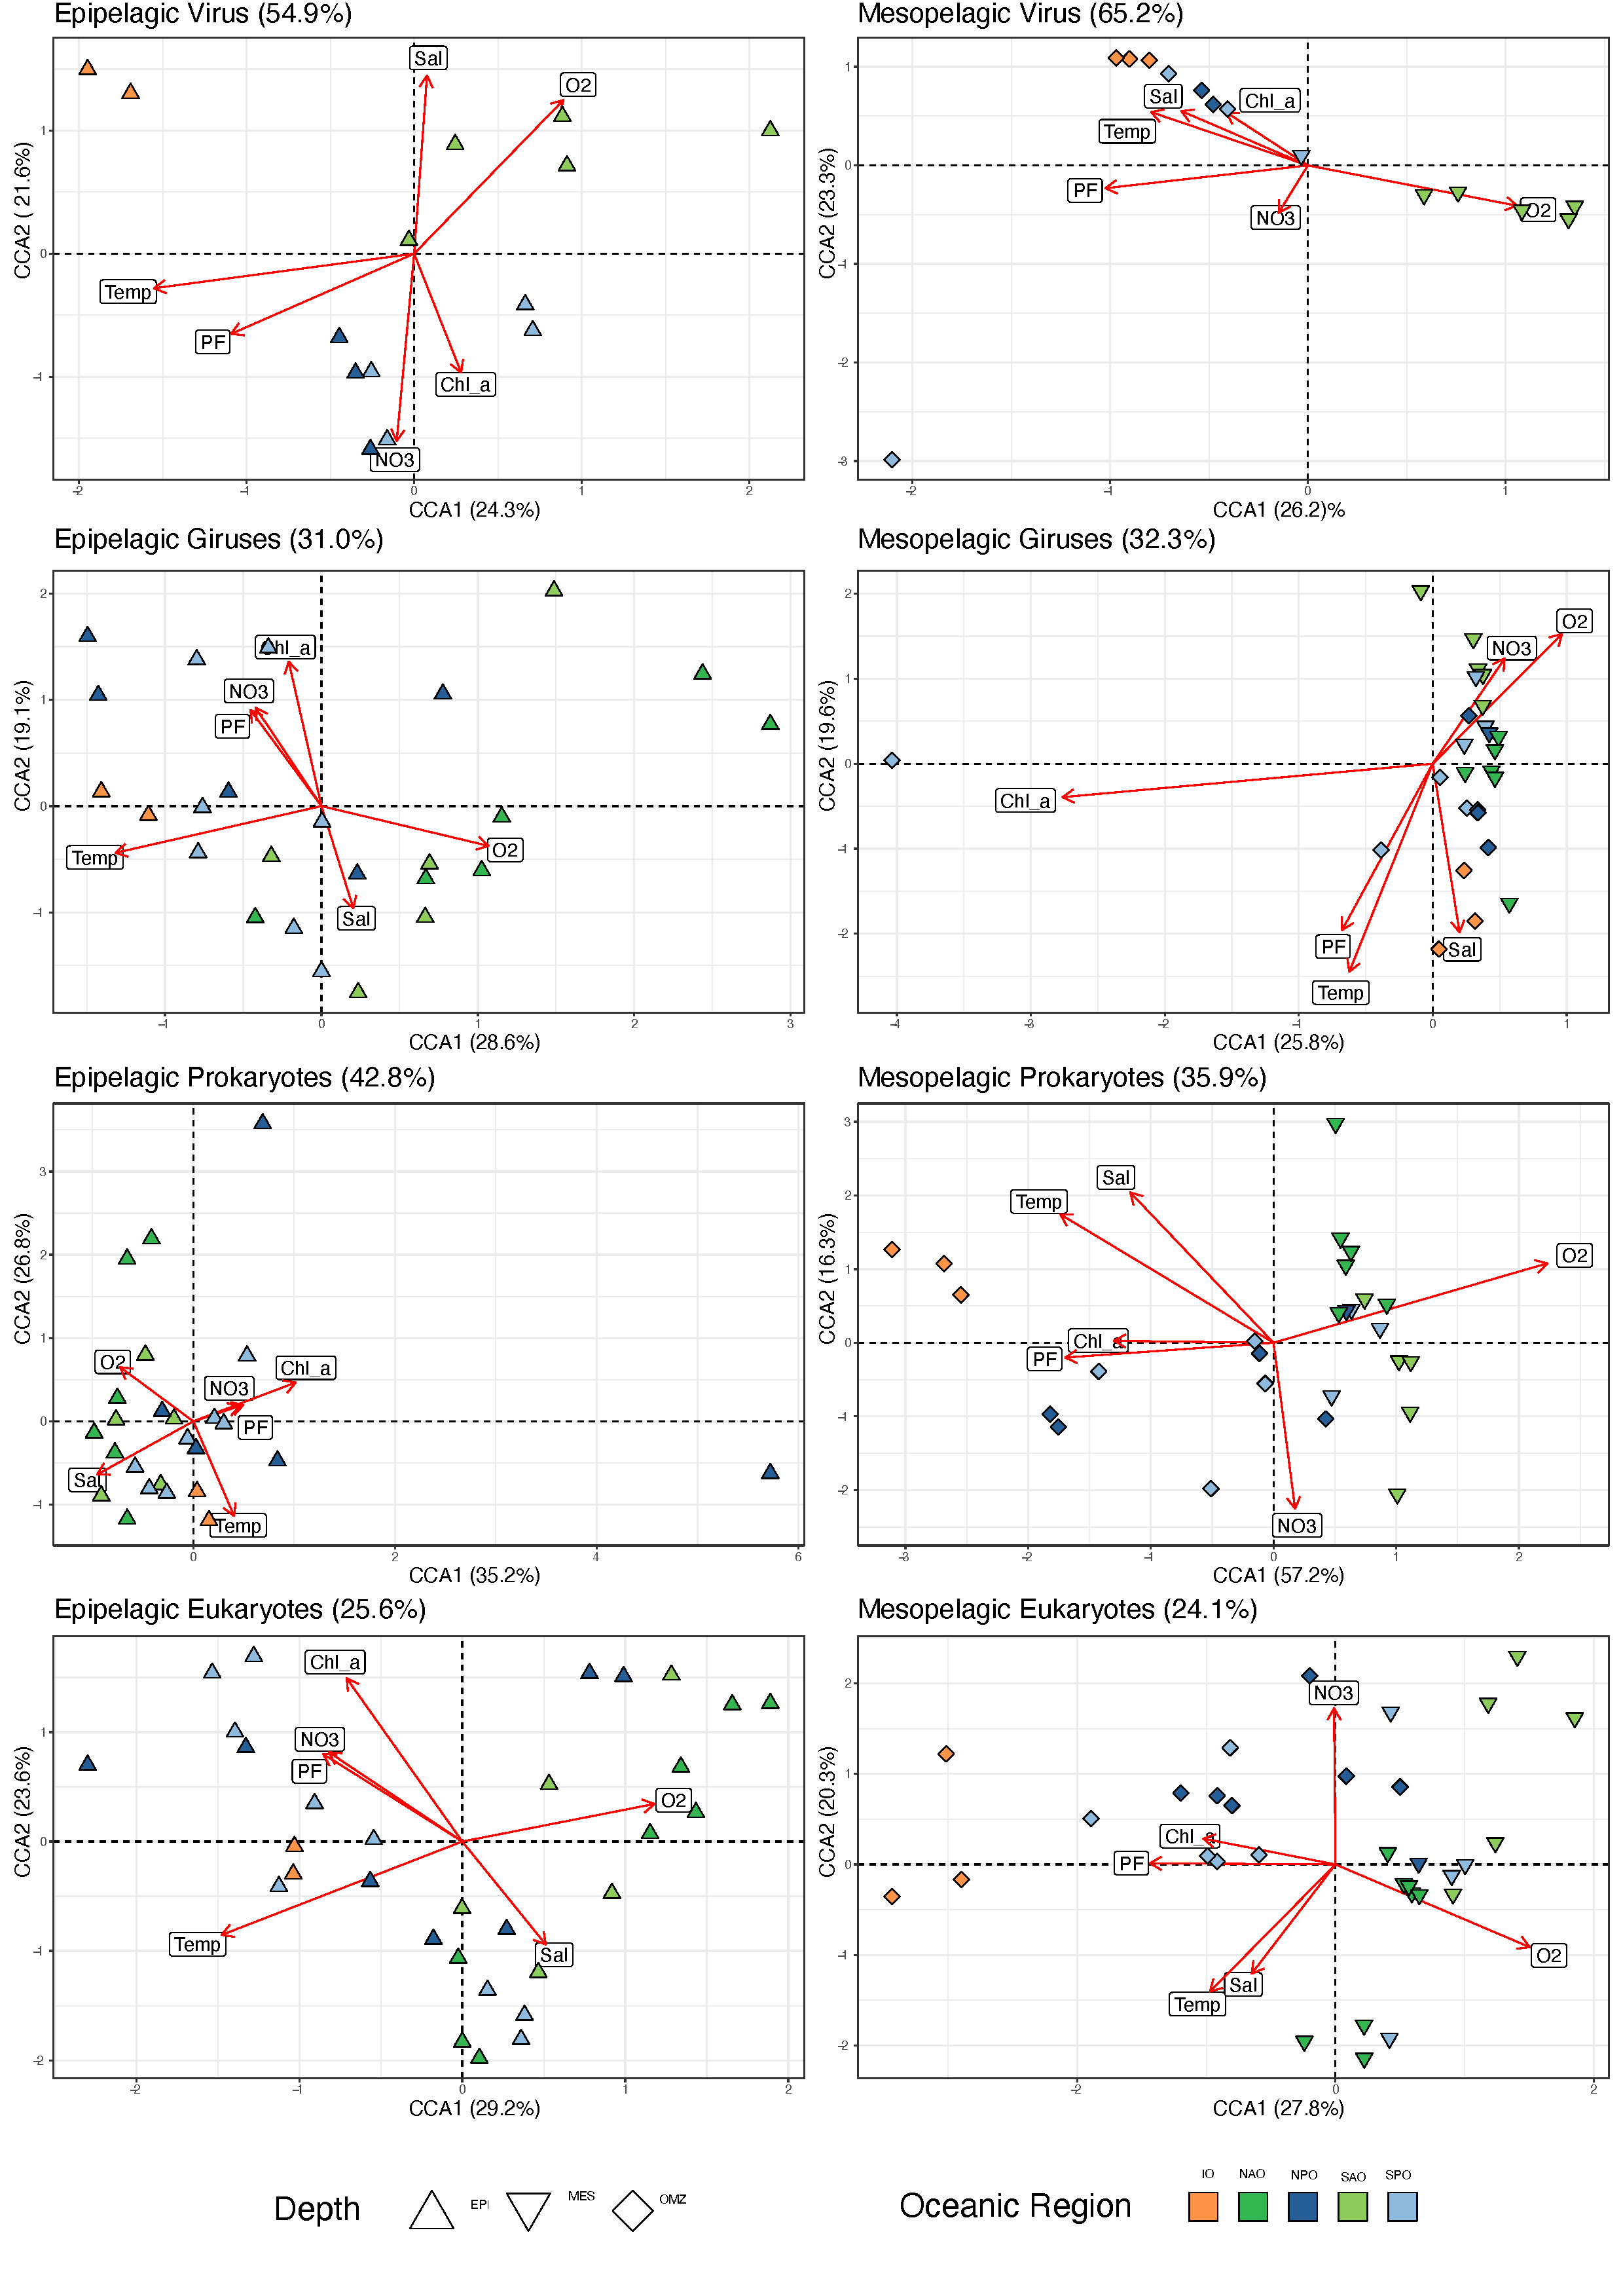
\includegraphics[scale=0.285]{images/custom_cca_plot_hellinger_no_bathy_labels_OS_regions_colors_to_print.pdf}
    \caption{Ordination plot of epipelagic and mesopelagic communities based on OTU’s composition canonical correspondence analysis (CCA), constrained by selected explanatory abiotic environmental parameters. IO: Indian Ocean, ...}
    \label{fig:cca_OS}
\end{figure}
\clearpage
\begin{figure}[ht]
    \centering
    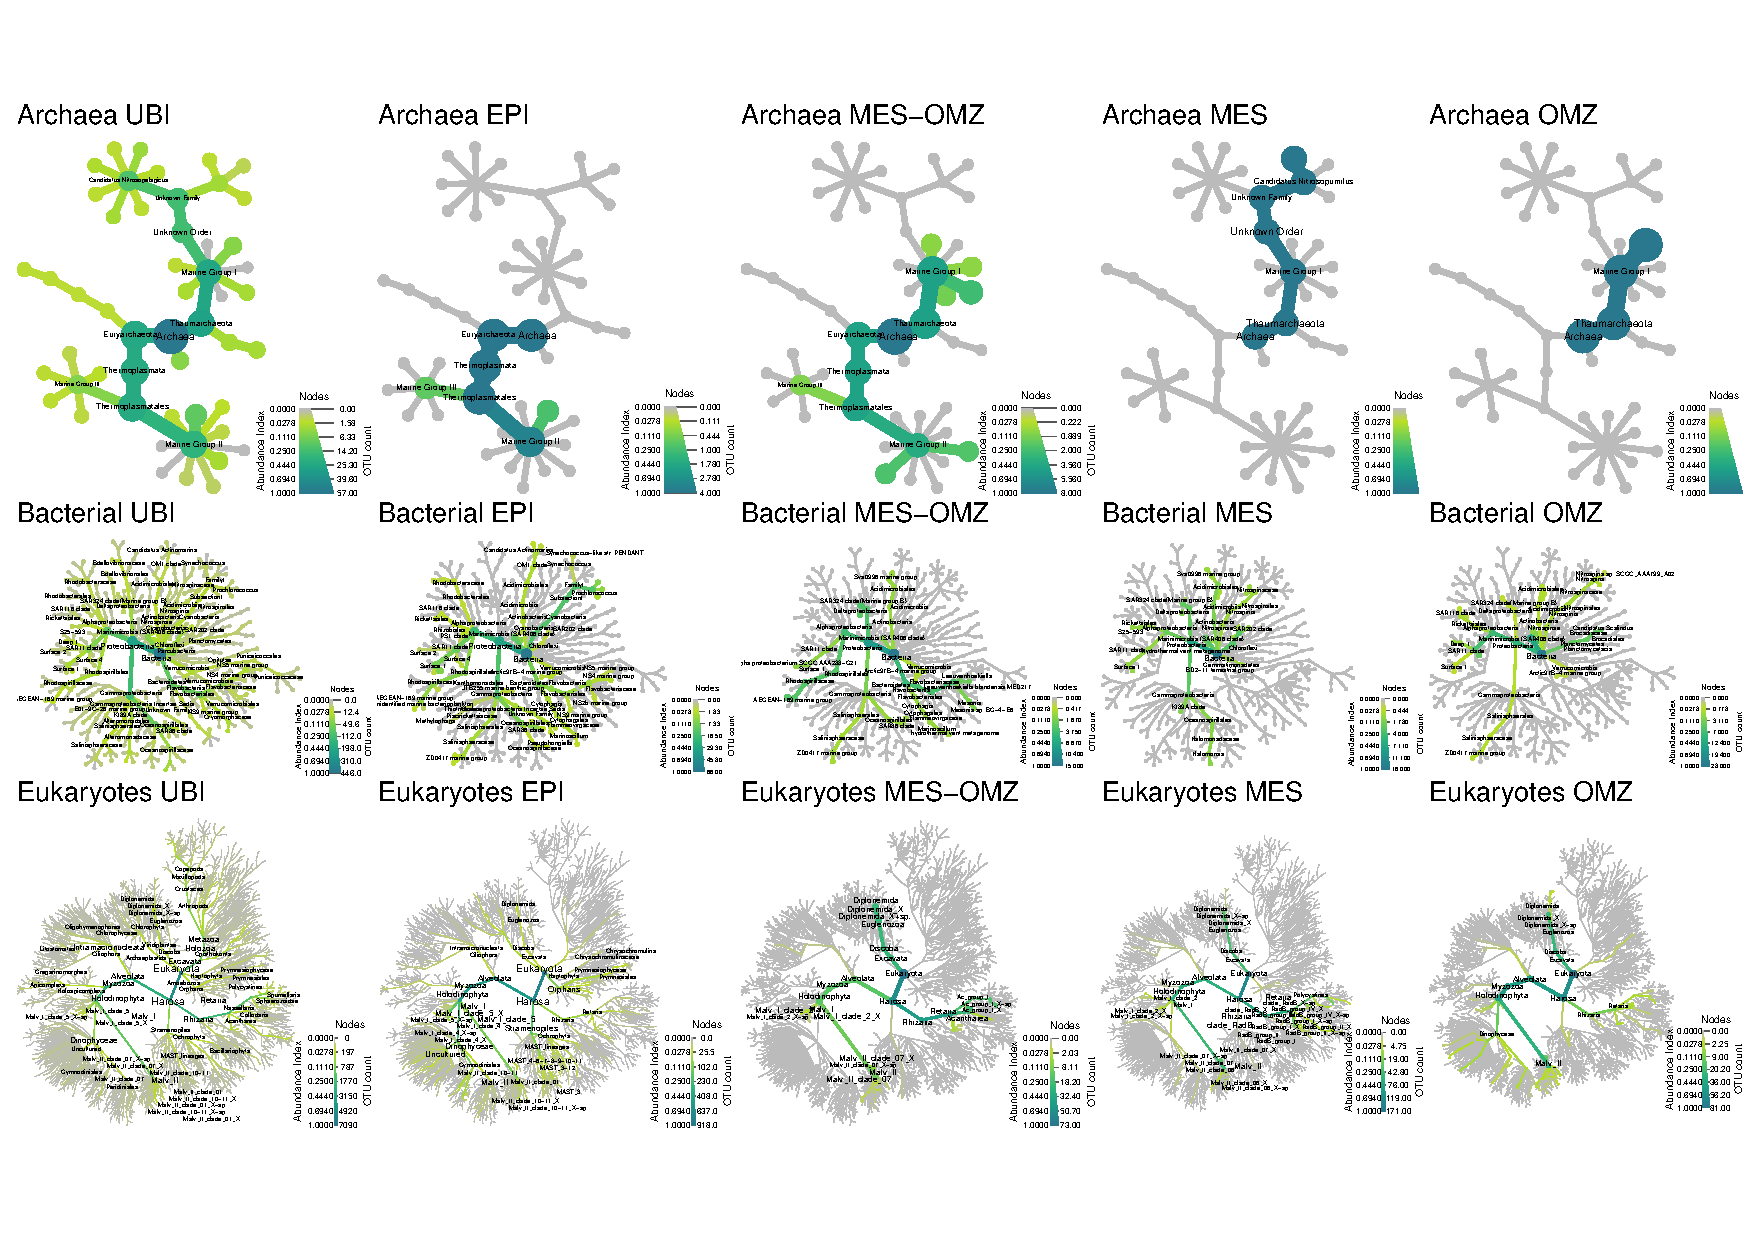
\includegraphics[scale=0.7,angle=90,origin=c]{images/hmap_general_pub.pdf}
    \caption{Taxonomy Trees}
    \label{fig:tax_trees}
\end{figure}
\clearpage
\begin{figure}[ht]
    \centering
    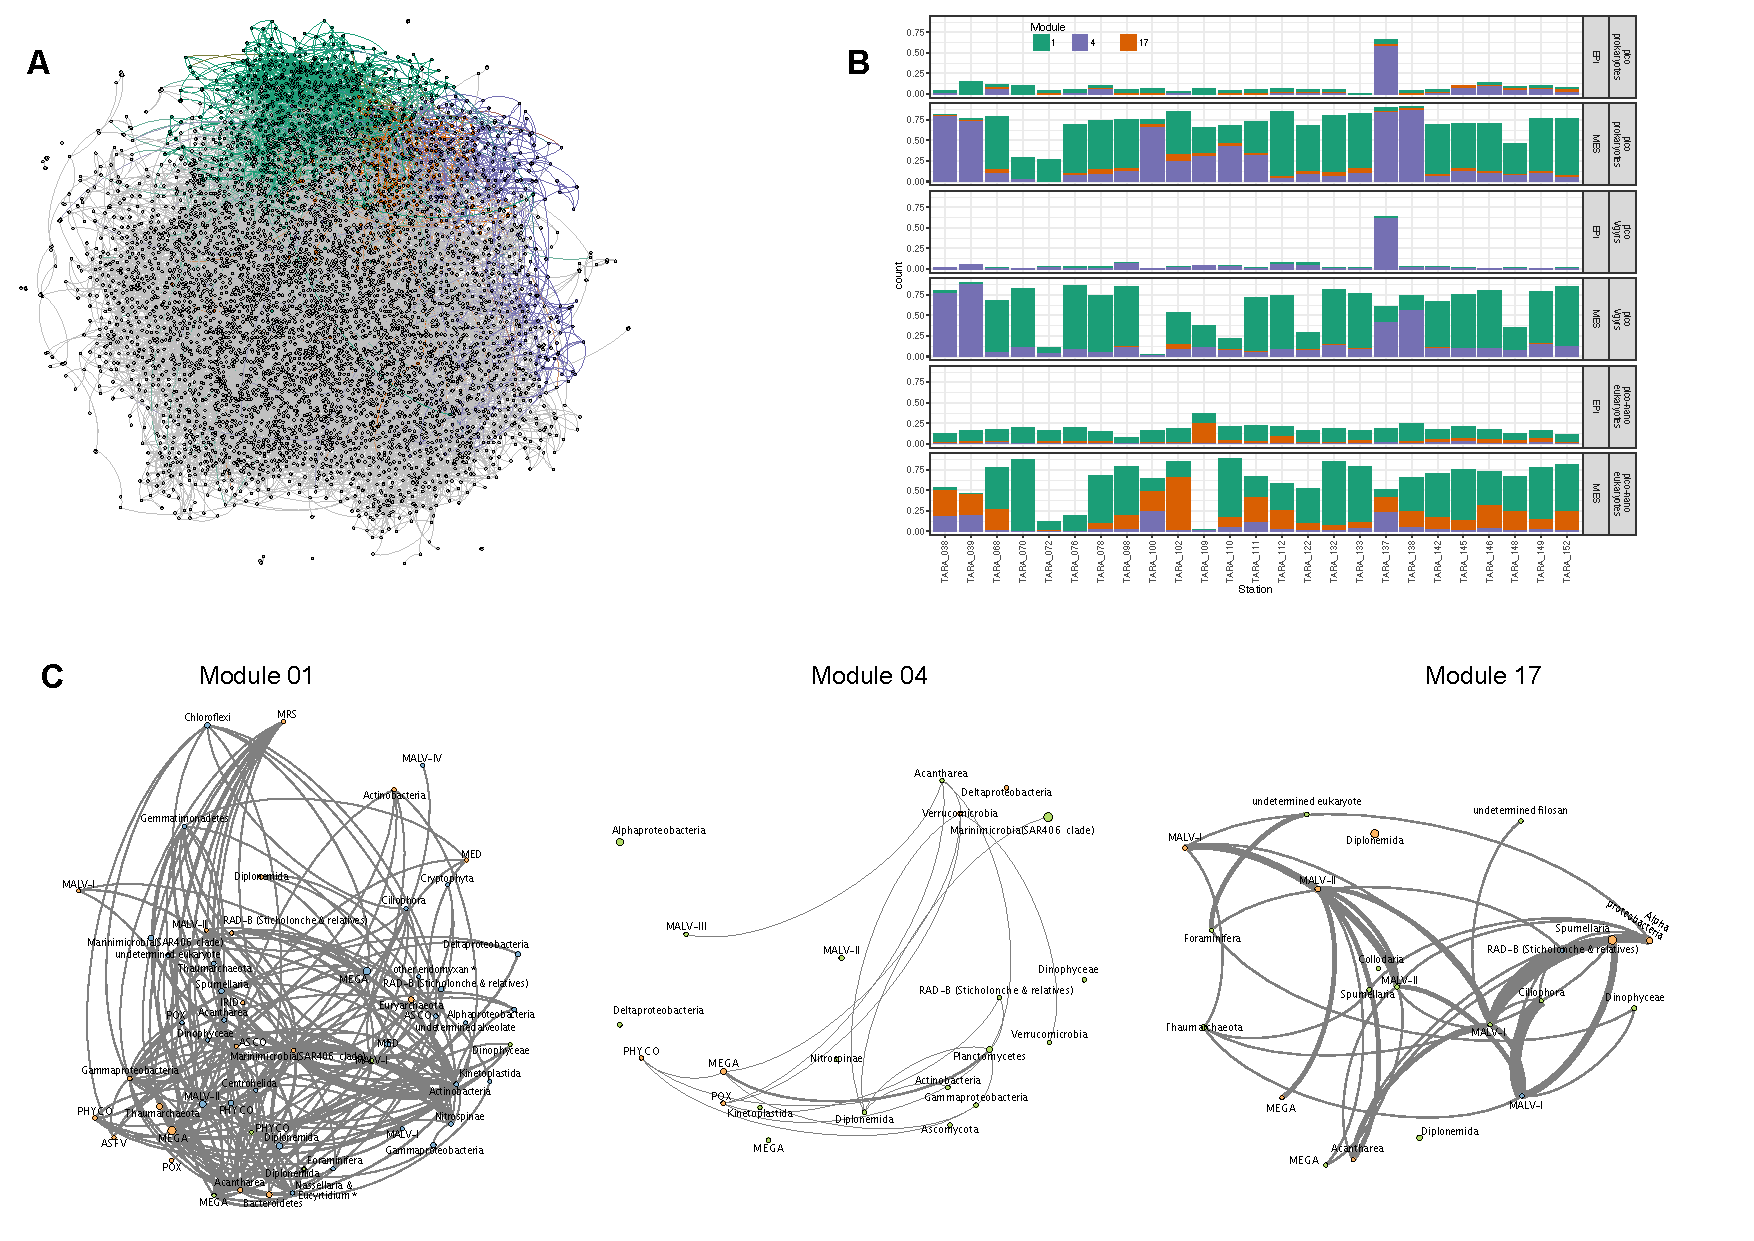
\includegraphics[scale=0.5]{images/Networks_Composite_v2.pdf}
    \caption{Co-Ocurrence Network between Epipelagic and Mesopelagic depth. A) Total Network, with connected modules for OMZ (purple and orange) and MES (green) highlighted. B) Relative taxa abundance in each Module in each Station and depth. C) Relative number of OTUs classified in broad taxonomic groups.}
    \label{fig:networks}
\end{figure}
\clearpage
\section*{Supplementary Figures}

\begin{suppfigure}[ht]
    \centering
    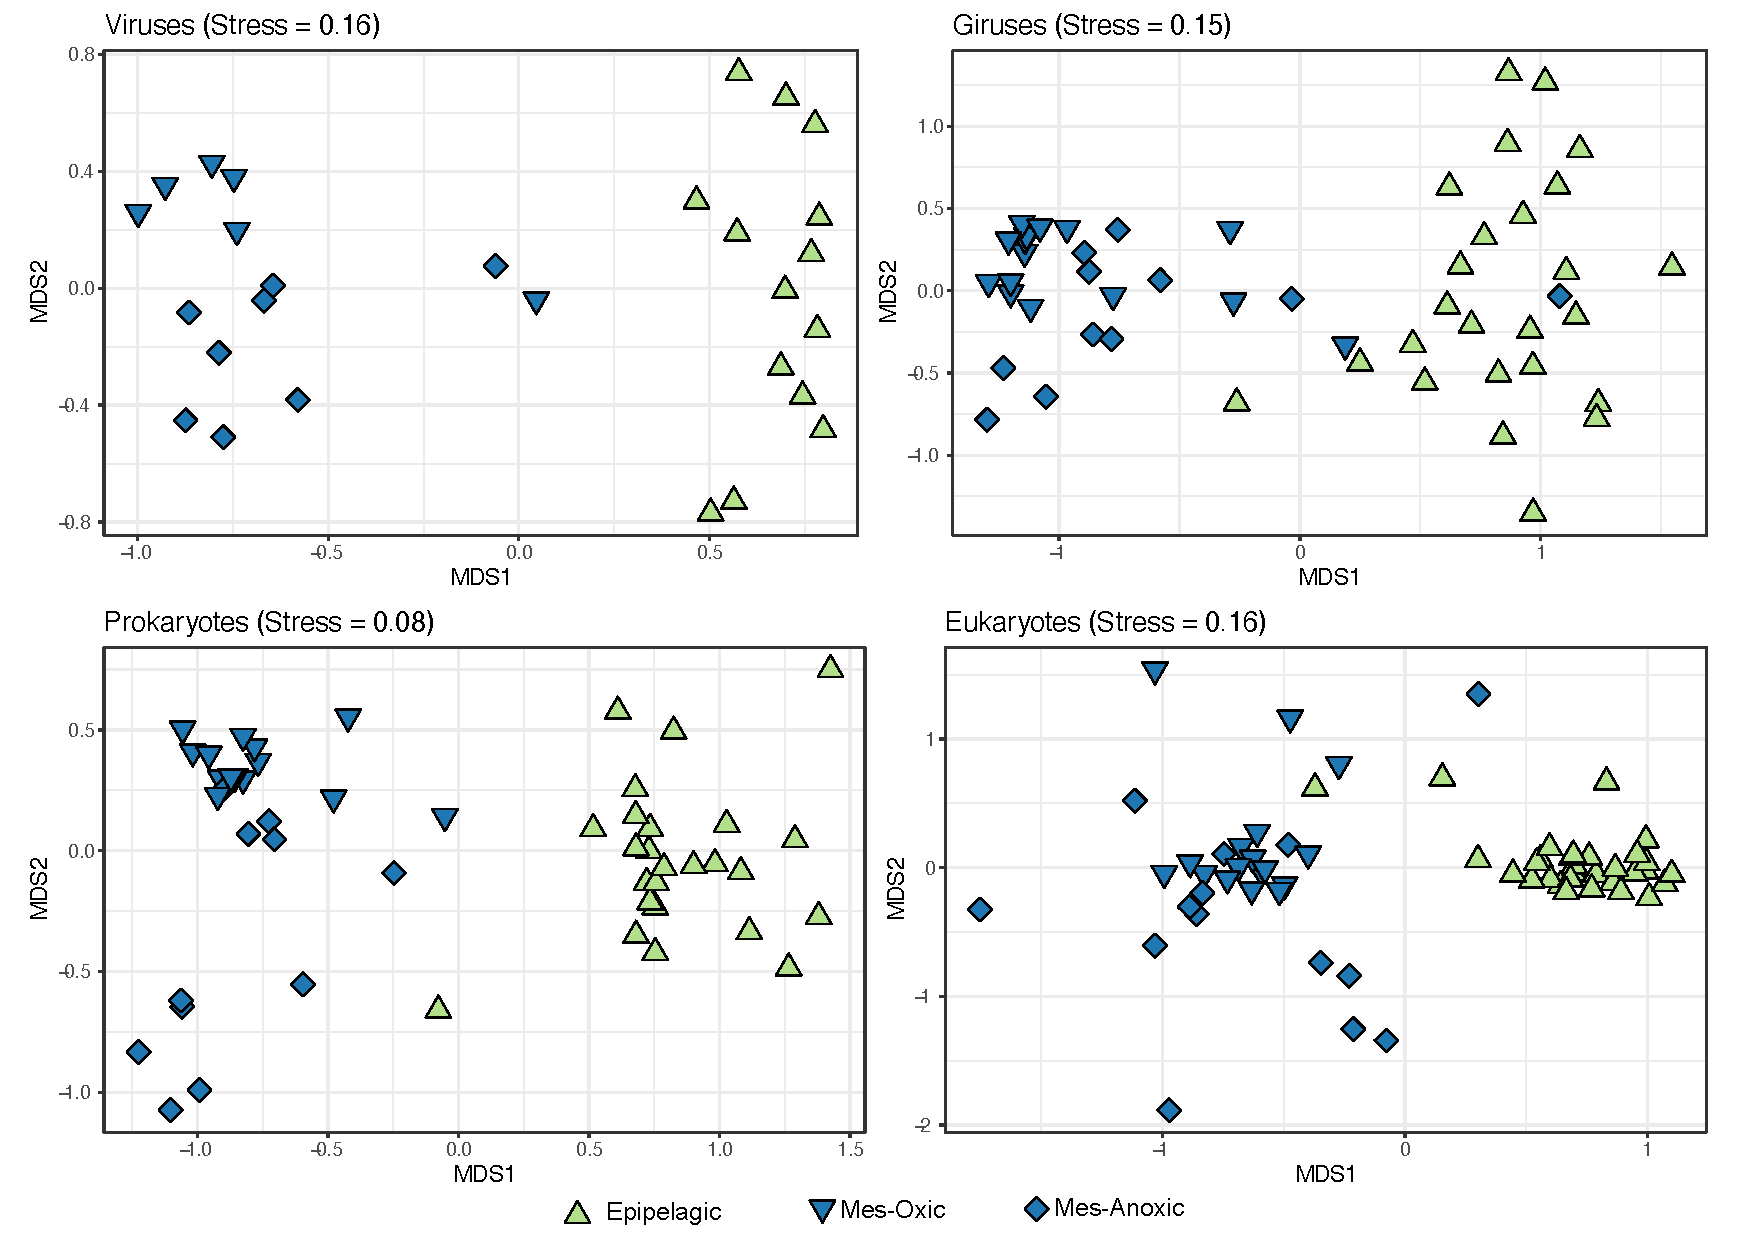
\includegraphics[scale=0.4]{images/nmds_used_SF_to_print.pdf}
    \caption{Non-metric multidimensional scaling (NMDS) for all samples demonstrating differences between epipelagic and mesopelagic communities in each organism group}
    \label{fig:nmds}
\end{suppfigure}
%\clearpage
\begin{suppfigure}[ht]
    \centering
    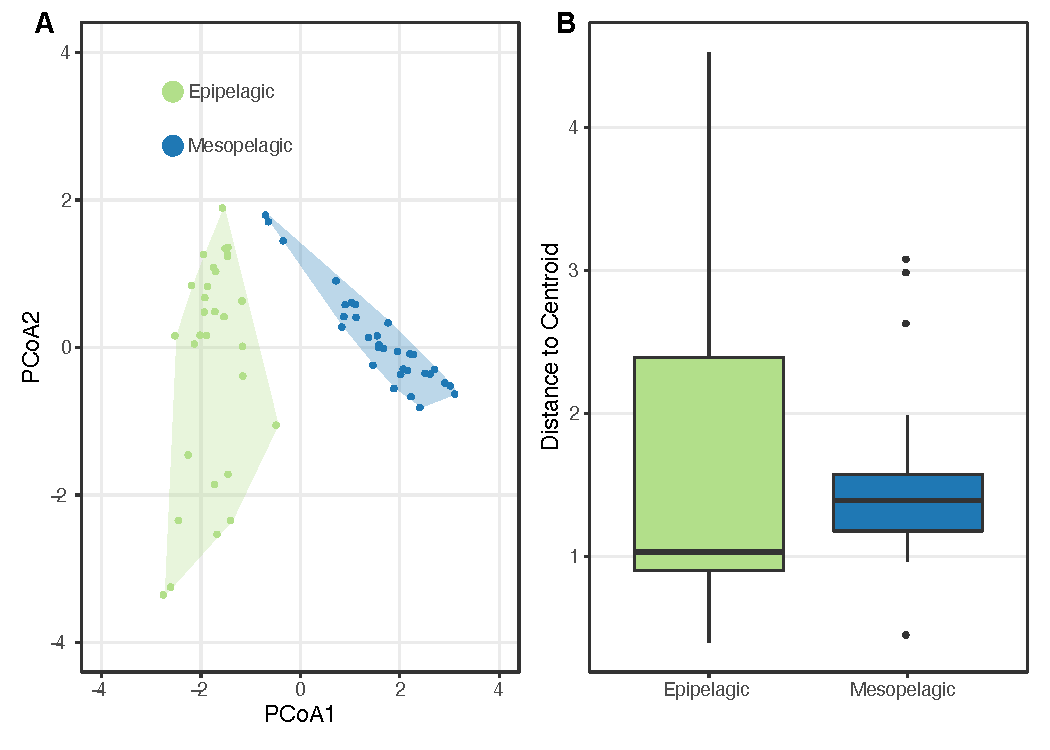
\includegraphics[scale=0.5]{images/betadisp_diganose_to_print.pdf}
    \caption{Epipelagic and mesopelagic group dispersions based on physical-chemical oceanic properties (Euclidian method). A) First two axes of PCoA. B) Dispersion of distances from Samples to Centroids.}
    \label{fig:betadipersion}
\end{suppfigure}
\clearpage
\begin{suppfigure}[ht]
    \centering
    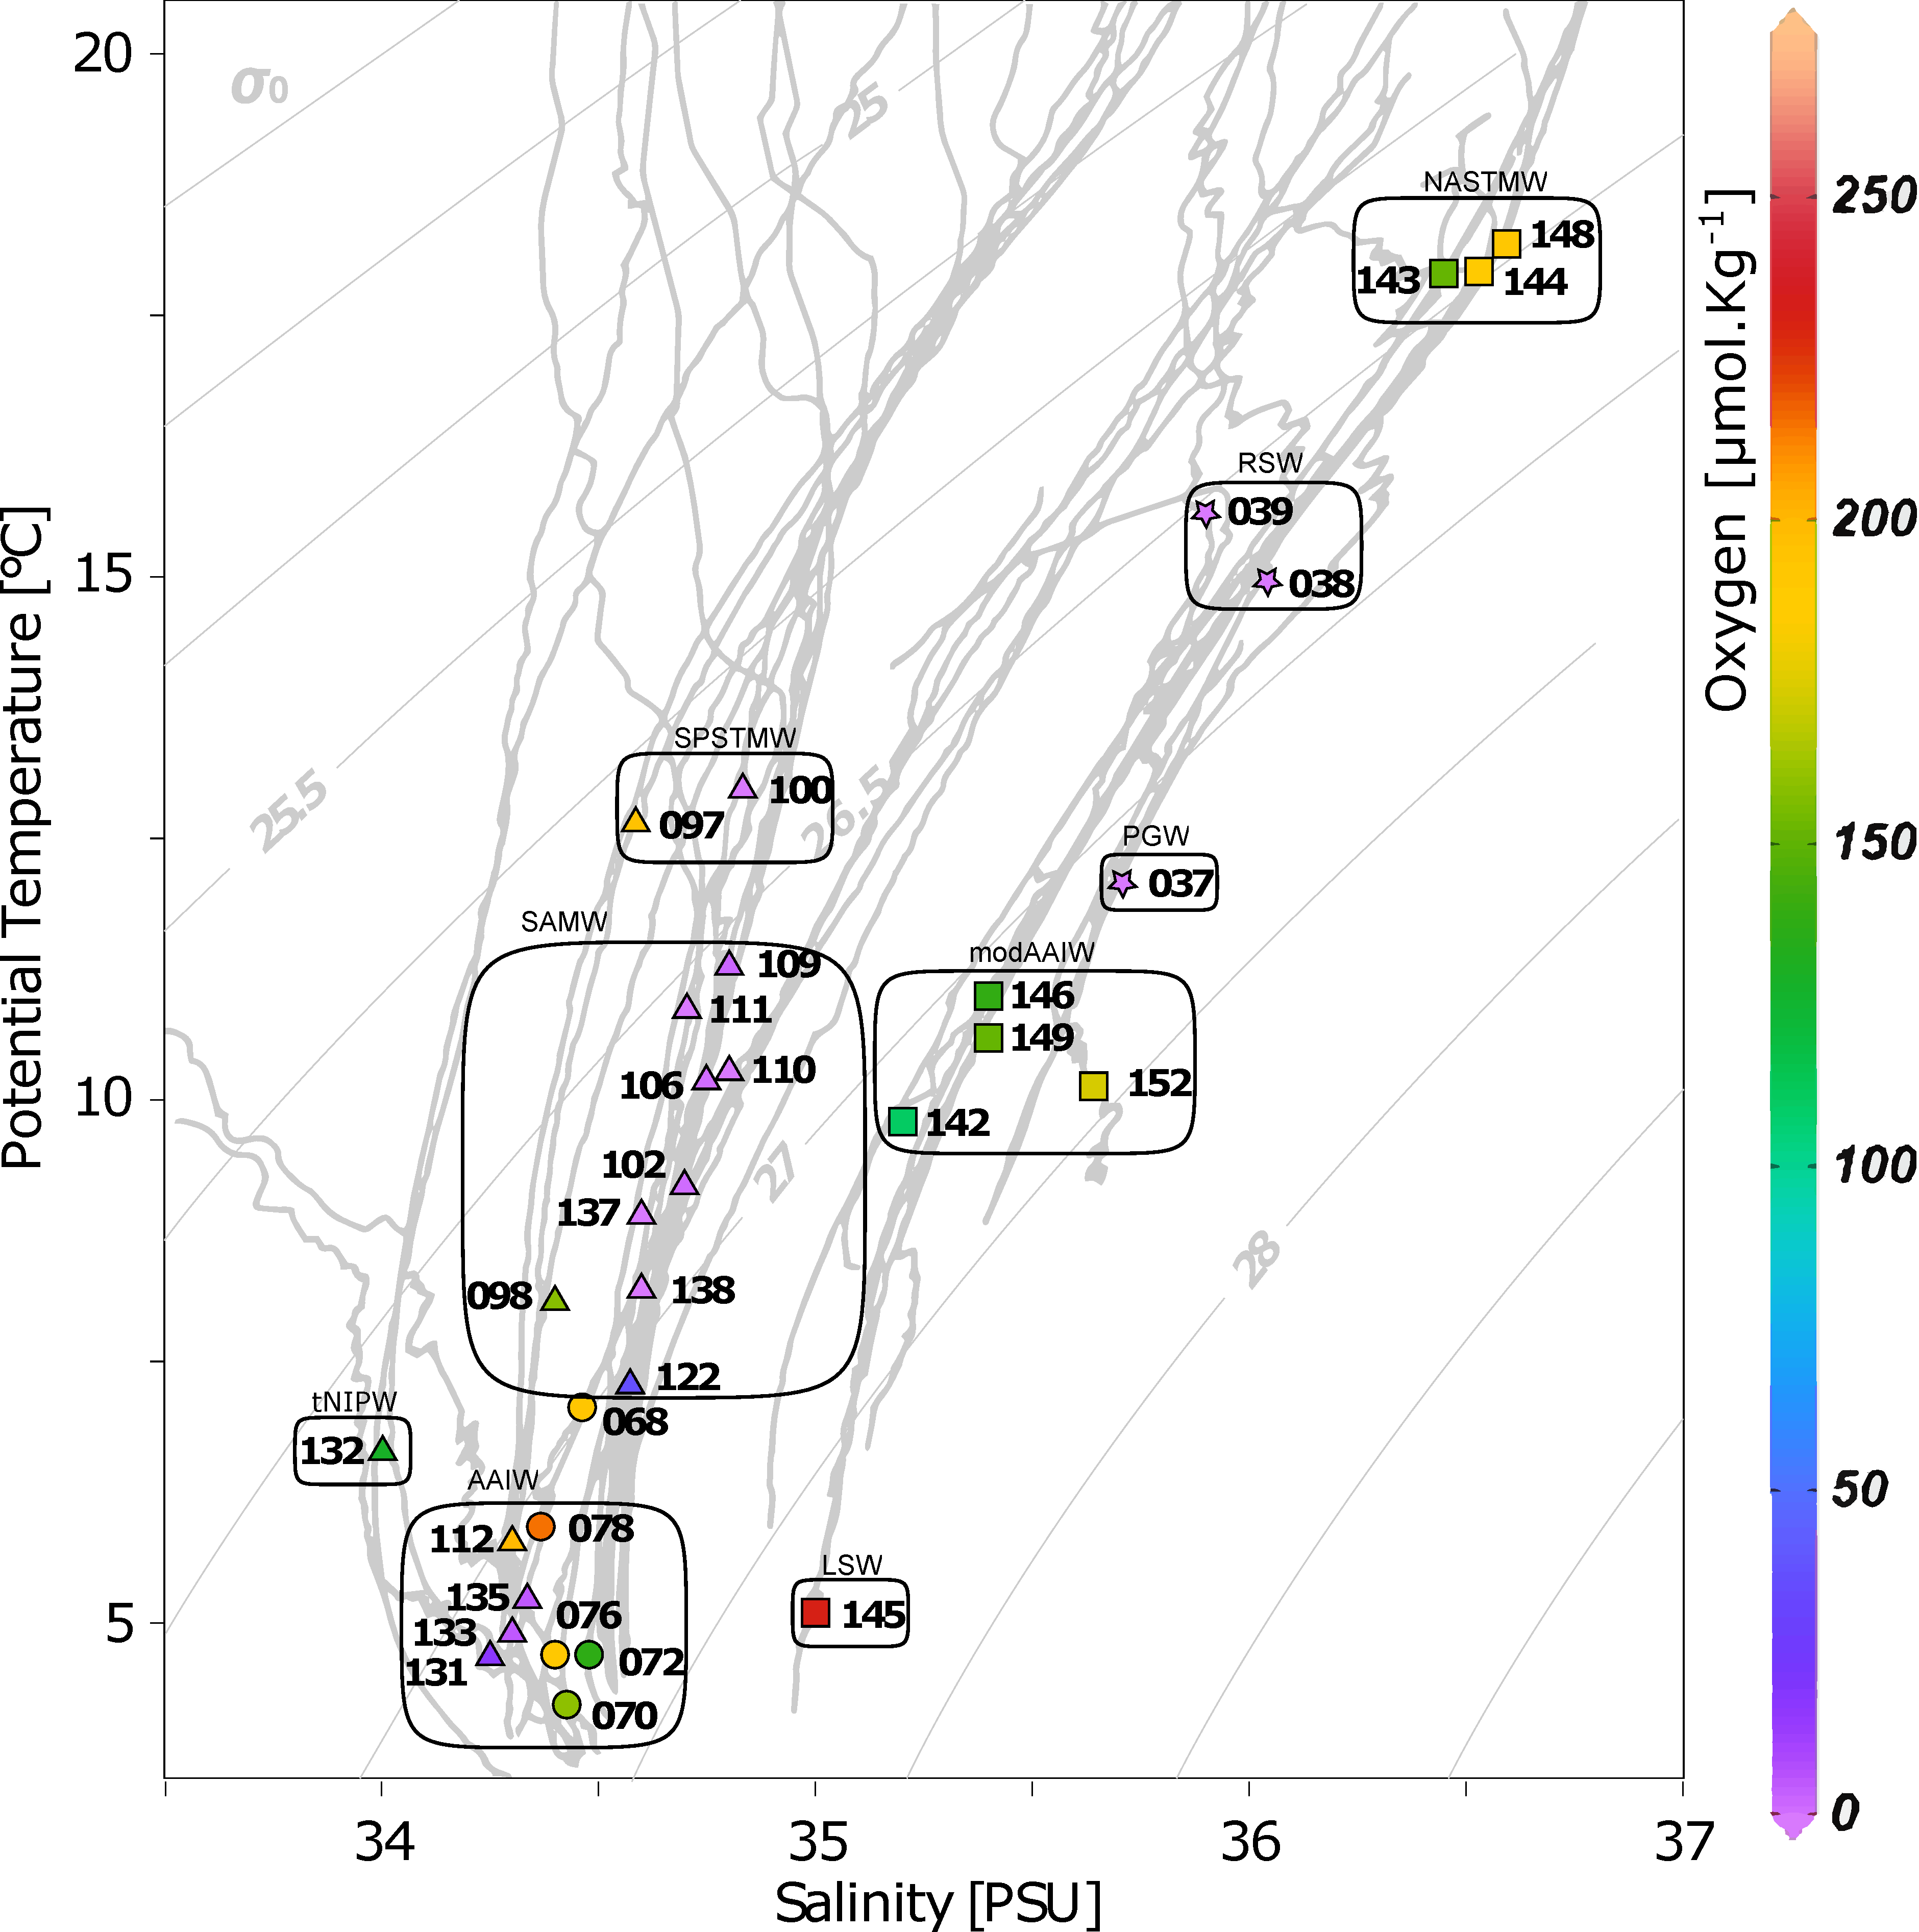
\includegraphics[scale=0.2]{images/T_Splot.pdf}
    \caption{Temperature and salinity plot indicating water mass properties for all mesopelagic samples. Formats represent the different oceanic basins ( $\Box$- North Atlantic Ocean, $\bigcirc$  - South Atlantic Ocean, $\bigtriangleup$ - Pacific Ocean, $\bigstar$ - Indian Ocean). Colours indicate the oxygen concentration at the sampling depth. LSW - Labrador Sea Water; AAIW - Antarctic Intermediate Water; tNPIW – transitional North Pacific Intermediate Water; SAMW - Subantarctic Mode Water; SPSTMW - South Pacific Subtropical Mode Water; modAAIW - modified Antarctic Intermediate Water; PGW - Persian Gulf Water mass; RSW - Red Sea Water mass; NASTMW - North Atlantic Subtropical Mode Water.}
    \label{fig:T_Splot}
\end{suppfigure}
\clearpage
\begin{suppfigure}[ht]
    \centering
    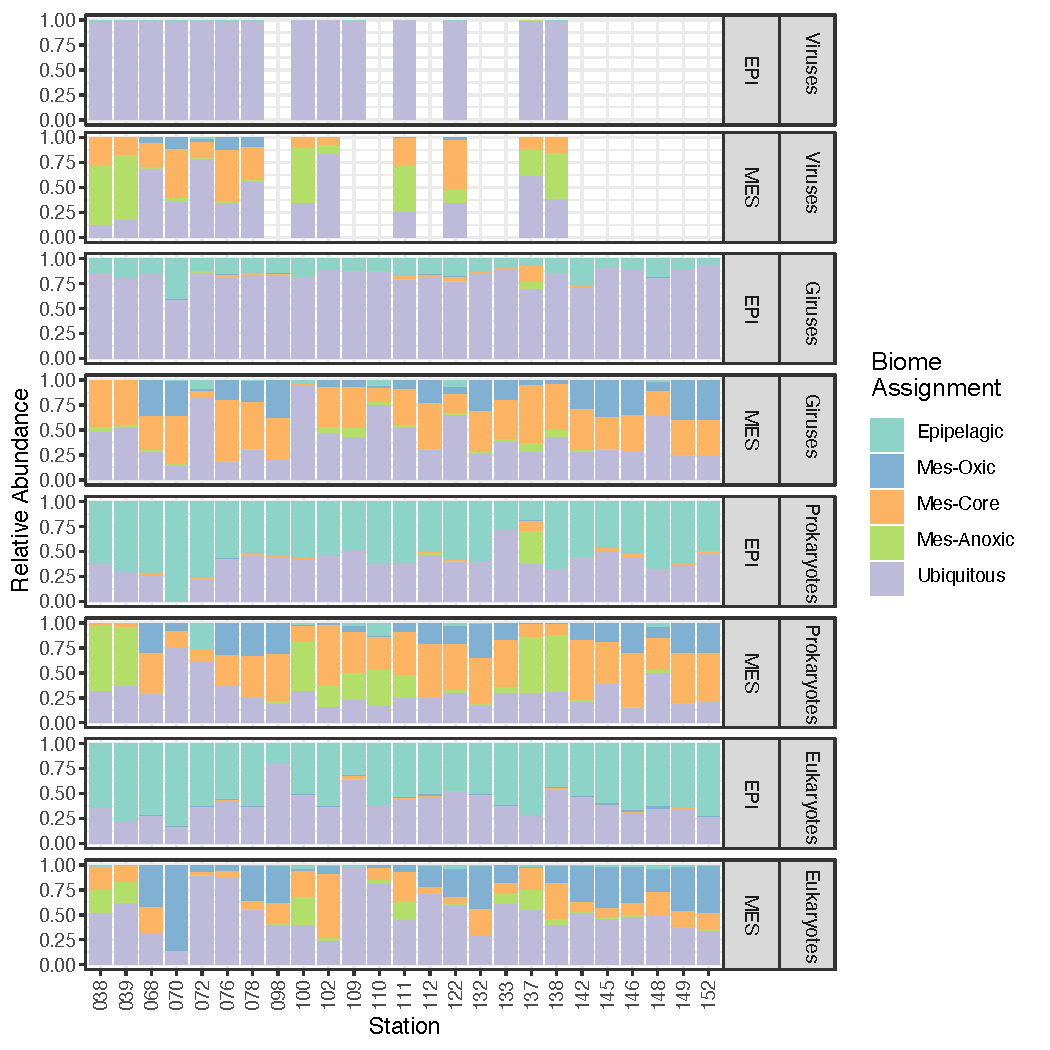
\includegraphics[scale=0.9]{images/simple_biome_projection_to_print.pdf}
    \caption{Biome Assignation}
    \label{fig:sim_biome}
\end{suppfigure}

\begin{suppfigure}[ht]
    \centering
    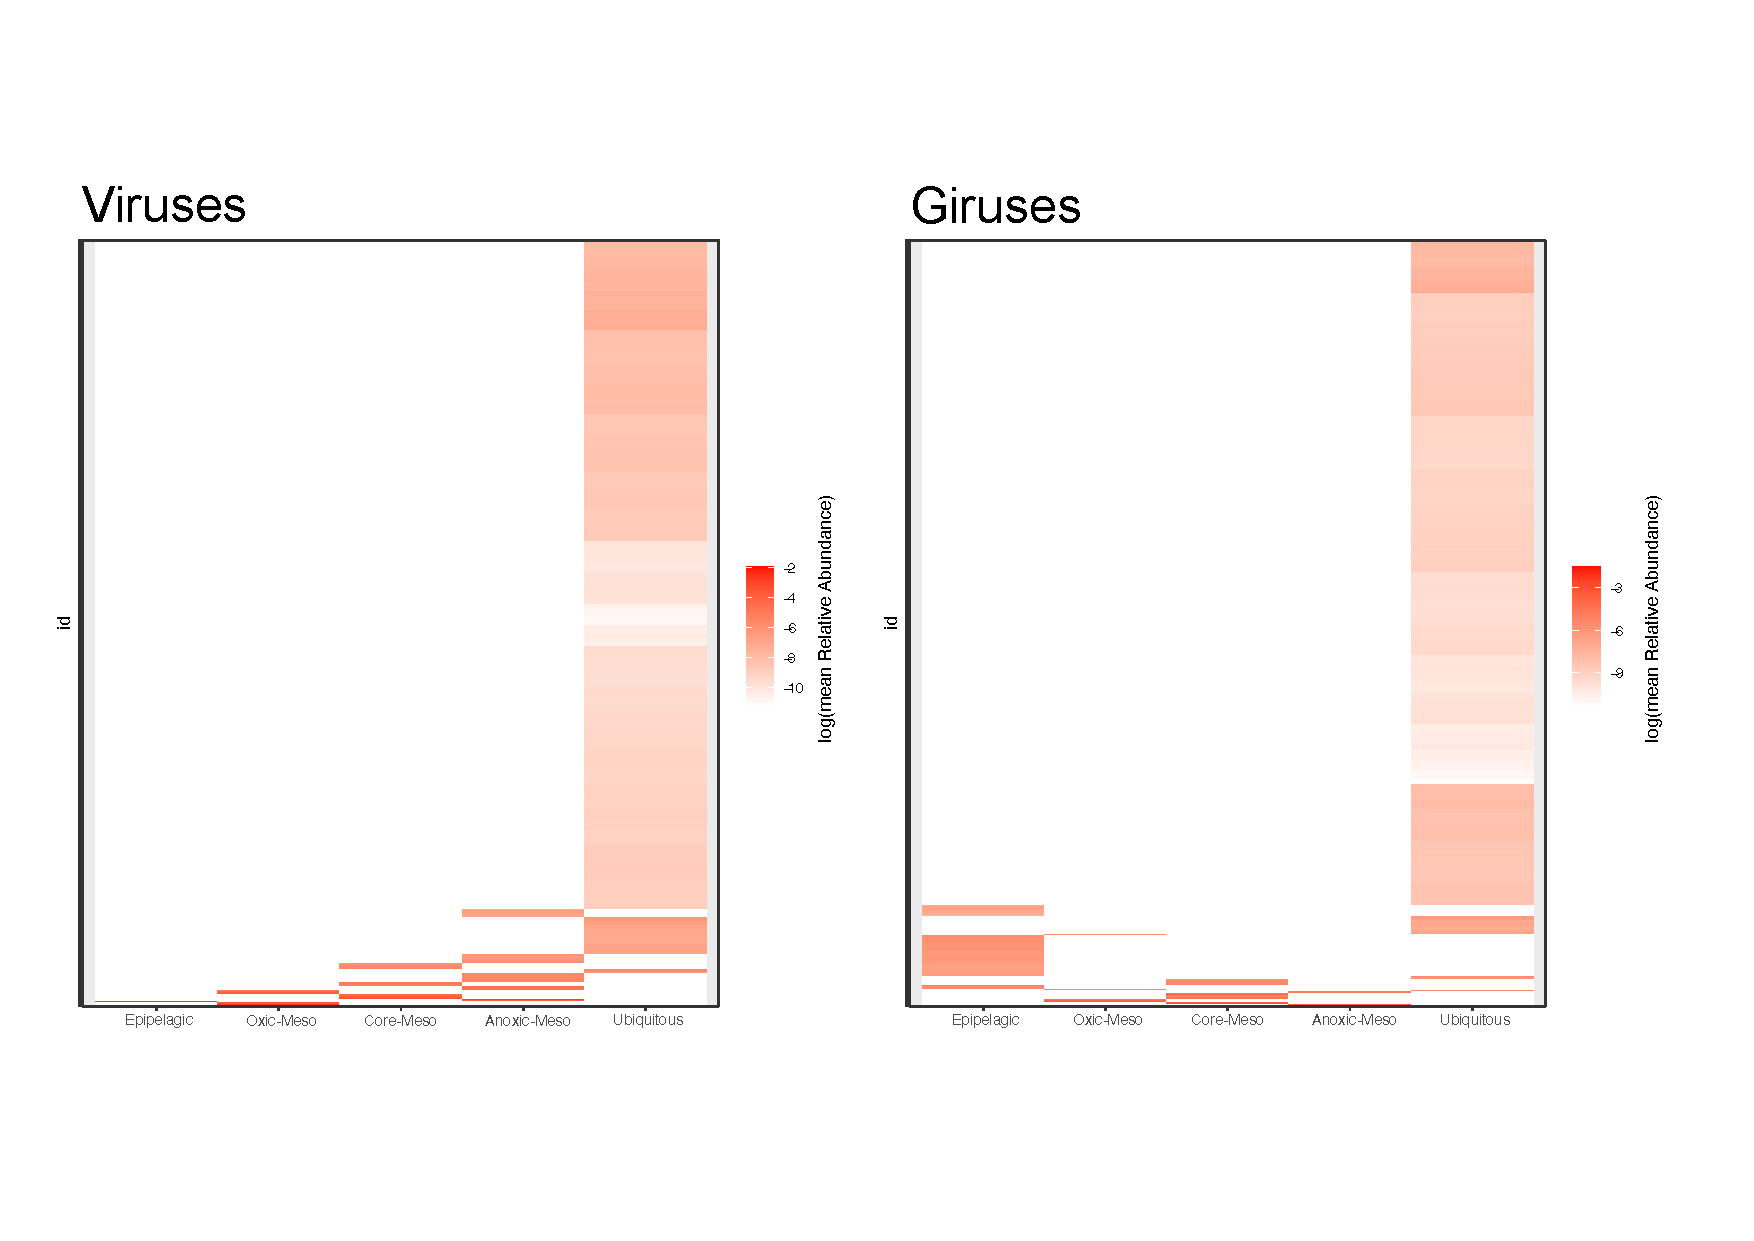
\includegraphics[scale=0.4]{images/heatmap_Vir_Gir.pdf}
    \caption{Virus / Girsues abundance heatmap}
    \label{fig:tax_virus_heatmap}
\end{suppfigure}

\begin{suppfigure}[ht]
    \centering
    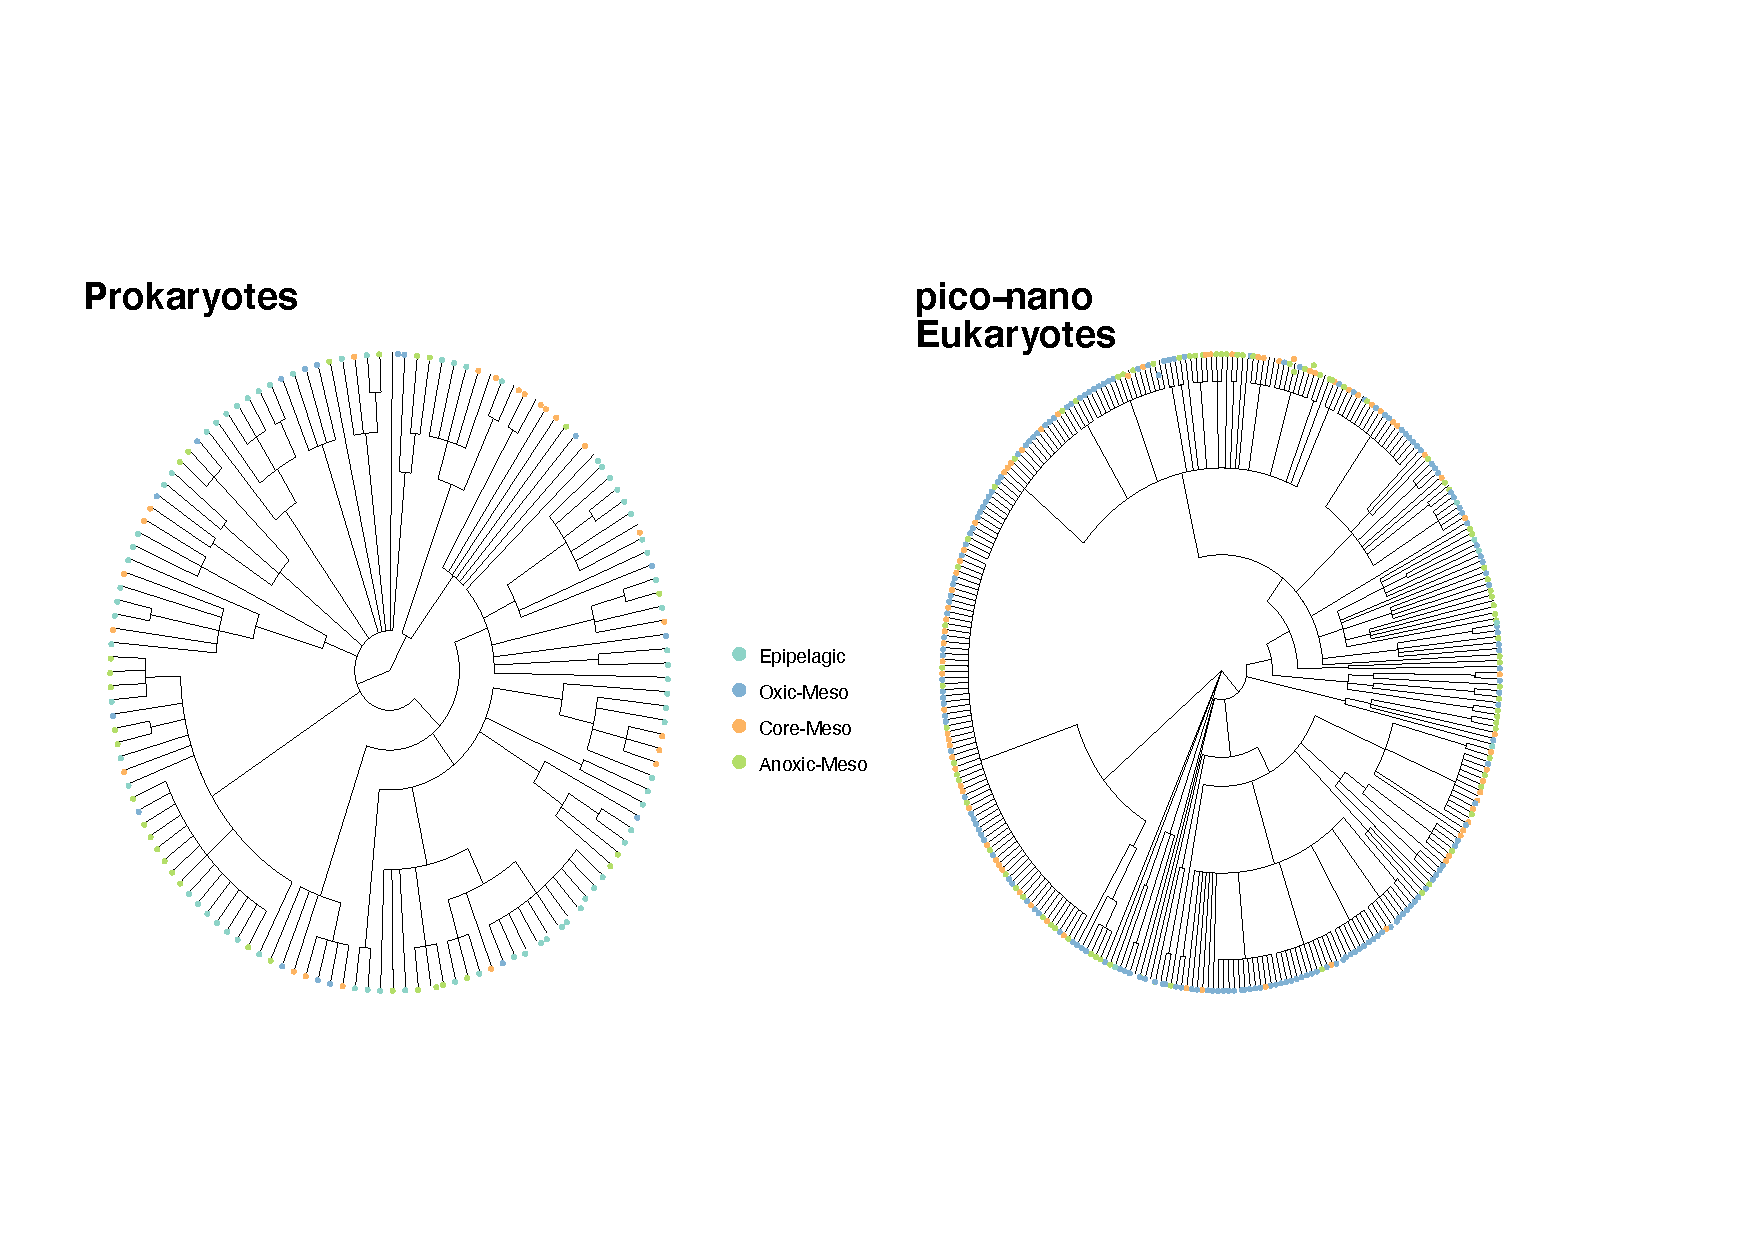
\includegraphics[scale=0.6,origin=c]{images/Trees_OTU_sup.pdf}
    \caption{Taxonomy Trees at OTU Level}
    \label{fig:tax_trees_sup}
\end{suppfigure}
\clearpage

%\subsection*{Subsection}
%
%Example text under a subsection. Bulleted lists may be used where appropriate, e.g.
%
%\begin{itemize}
%\item First item
%\item Second item
%\end{itemize}
%
%\subsubsection*{Third-level section}
% 
%Topical subheadings are allowed.
%
%\section*{Data Records}
%
%The Data Records section should be used to explain each data record associated with this work, including the repository where this information is stored, and to provide an overview of the data files and their formats. Each external data record should be cited numerically in the text of this section, for example \cite{Hao:gidmaps:2014}, and included in the main reference list as described below. A data citation should also be placed in the subsection of the Methods containing the data-collection or analytical procedure(s) used to derive the corresponding record. Providing a direct link to the dataset may also be helpful to readers (\hyperlink{https://doi.org/10.6084/m9.figshare.853801}{https://doi.org/10.6084/m9.figshare.853801}).
%
%Tables should be used to support the data records, and should clearly indicate the samples and subjects (study inputs), their provenance, and the experimental manipulations performed on each (please see 'Tables' below). They should also specify the data output resulting from each data-collection or analytical step, should these form part of the archived record.
%
%\section*{Technical Validation}
%
%This section presents any experiments or analyses that are needed to support the technical quality of the dataset. This section may be supported by figures and tables, as needed. This is a required section; authors must present information justifying the reliability of their data.
%
%\section*{Usage Notes}
%
%The Usage Notes should contain brief instructions to assist other researchers with reuse of the data. This may include discussion of software packages that are suitable for analysing the assay data files, suggested downstream processing steps (e.g. normalization, etc.), or tips for integrating or comparing the data records with other datasets. Authors are encouraged to provide code, programs or data-processing workflows if they may help others understand or use the data. Please see our code availability policy for advice on supplying custom code alongside Data Descriptor manuscripts.
%
%For studies involving privacy or safety controls on public access to the data, this section should describe in detail these controls, including how authors can apply to access the data, what criteria will be used to determine who may access the data, and any limitations on data use. 
%
%\section*{Code availability}
%
%For all studies using custom code in the generation or processing of datasets, a statement must be included under the heading "Code availability", indicating whether and how the code can be accessed, including any restrictions to access. This section should also include information on the versions of any software used, if relevant, and any specific variables or parameters used to generate, test, or process the current dataset. 



\bibliography{MesoLibrary_2}

\section*{Acknowledgements} (not compulsory)

Acknowledgements should be brief, and should not include thanks to anonymous referees and editors, or effusive comments. Grant or contribution numbers may be acknowledged.

This study is part of the “Ocean Plankton, Climate and Development” project funded by the French Facility for Global Environment (FFEM). Rigonato J., Budinich B., Murillo A.A., Pierella Karlusich J.J., Brandão M.C. and Soviadan Y.D. received financial support from FFEM to execute the project. Brandão, M.C. also received financial support from Coordination for the Improvement of Higher Education Personnel of Brazil (CAPES 99999.000487/2016-03). We acknowledge Noan Le Bescot (Ternog Design) for assistance in preparing figures. Tara Oceans (which includes both the Tara Oceans and Tara Oceans Polar Circle expeditions) would not exist without the leadership of the Tara Expeditions Foundation and the continuous support of 23 institutes (http://oceans.taraexpeditions.org). We further thank the commitment of the following sponsors: CNRS (in particular Groupement de Recherche GDR3280 and the Research Federation for the study of Global Ocean Systems Ecology and Evolution, FR2022/Tara Oceans-GOSEE), European Molecular Biology Laboratory (EMBL), Genoscope/CEA, The French Ministry of Research, and the French Government ‘Investissements d’Avenir’ programmes OCEANOMICS (ANR-11-BTBR-0008), FRANCE GENOMIQUE (ANR-10-INBS-09-08), MEMO LIFE (ANR-10-LABX-54), and PSL* Research University (ANR-11-IDEX-0001-02). We also thank the support and commitment of agnès b. and Etienne Bourgois, the Prince Albert II de Monaco Foundation, the Veolia Foundation, Region Bretagne, Lorient Agglomeration, Serge Ferrari, World Courier, and KAUST. The global sampling effort was enabled by countless scientists and crew who sampled aboard the Tara from 2009-2013, and we thank MERCATOR-CORIOLIS and ACRI-ST for providing daily satellite data during the expeditions. We are also grateful to the countries who graciously granted sampling permission. The authors declare that all data reported herein are fully and freely available from the date of publication, with no restrictions, and that all of the analyses, publications, and ownership of data are free from legal entanglement or restriction by the various nations whose waters the Tara Oceans expeditions sampled in. This article is contribution number XX of Tara Oceans.

%\section*{Author contributions statement}

%Must include all authors, identified by initials, for example:
%A.A. conceived the experiment(s), A.A. and B.A. conducted the experiment(s), C.A. and D.A. analysed the results. All authors reviewed the manuscript. 

%\section*{Competing interests} (mandatory statement)

%The corresponding author is responsible for providing a \href{https://www.nature.com/sdata/policies/editorial-and-publishing-policies#competing}{competing interests statement} on behalf of all authors of the paper. This statement must be included in the submitted article file.

%\section*{Figures \& Tables}


%\begin{table}[ht]
%\centering
%\begin{tabular}{|l|l|l|}
%\hline
%Condition & n & p \\
%\hline
%A & 5 & 0.1 \\
%\hline
%B & 10 & 0.01 \\
%\hline
%\end{tabular}
%\caption{\label{tab:example}Legend (350 words max). Example legend text.}
%\end{table}

\end{document}